% This is "sig-alternate.tex" V1.9 April 2009
% This file should be compiled with V2.4 of "sig-alternate.cls" April 2009
%
% This example file demonstrates the use of the 'sig-alternate.cls'
% V2.4 LaTeX2e document class file. It is for those submitting
% articles to ACM Conference Proceedings WHO DO NOT WISH TO
% STRICTLY ADHERE TO THE SIGS (PUBS-BOARD-ENDORSED) STYLE.
% The 'sig-alternate.cls' file will produce a similar-looking,
% albeit, 'tighter' paper resulting in, invariably, fewer pages.
%
% ----------------------------------------------------------------------------------------------------------------
% This .tex file (and associated .cls V2.4) produces:
%       1) The Permission Statement
%       2) The Conference (location) Info information
%       3) The Copyright Line with ACM data
%       4) NO page numbers
%
% as against the acm_proc_article-sp.cls file which
% DOES NOT produce 1) thru' 3) above.
%
% Using 'sig-alternate.cls' you have control, however, from within
% the source .tex file, over both the CopyrightYear
% (defaulted to 200X) and the ACM Copyright Data
% (defaulted to X-XXXXX-XX-X/XX/XX).
% e.g.
% \CopyrightYear{2007} will cause 2007 to appear in the copyright line.
% \crdata{0-12345-67-8/90/12} will cause 0-12345-67-8/90/12 to appear in the copyright line.
%
% ---------------------------------------------------------------------------------------------------------------
% This .tex source is an example which *does* use
% the .bib file (from which the .bbl file % is produced).
% REMEMBER HOWEVER: After having produced the .bbl file,
% and prior to final submission, you *NEED* to 'insert'
% your .bbl file into your source .tex file so as to provide
% ONE 'self-contained' source file.
%
% ================= IF YOU HAVE QUESTIONS =======================
% Questions regarding the SIGS styles, SIGS policies and
% procedures, Conferences etc. should be sent to
% Adrienne Griscti (griscti@acm.org)
%
% Technical questions _only_ to
% Gerald Murray (murray@hq.acm.org)
% ===============================================================
%
% For tracking purposes - this is V1.9 - April 2009

\documentclass{sig-alternate}
\usepackage{url}
\usepackage{algorithm}
\usepackage[noend]{algorithmic}
\usepackage{subfigure}

%\documentclass{acm_proc_article-sp}
%\def\BibTeX{Bib\TeX}
%\parindent=0pt
%\parskip=\baselineskip

\newcommand{\dae}{{\em Divide-and-Evolve}}
\newcommand{\DAEX}{{\sc DaE$_{\text{X}}$}}
\newcommand{\DAEYAHSP}{{\sc DaE$_{\text{YAHSP}}$}}
\newcommand{\YAHSP}{{\sc YAHSP}}

\def\UU{{\mathbb{U}}}


\begin{document}

%\title{A Multicore Implementation of the Divide-and-Evolve Algorithm}
%\title{Speeding Up the Individual Evaluation of the Divide-and-Evolve Algorithm}
%\title{Multithreading the Divide-and-Evolve Algorithm for a Multicore Machine}
%\title{A Multithreaded Release of the Divide-and-Evolve Planning System for a Multicore Machine}
%\title{A Multicore Implementation of the Individual Evaluation in the Divide-and-Evolve Planner}
\title{Parallel Divide-and-Evolve: Experiments with OpenMP on a Multicore Machine}


%
% You need the command \numberofauthors to handle the 'placement
% and alignment' of the authors beneath the title.
%
% For aesthetic reasons, we recommend 'three authors at a time'
% i.e. three 'name/affiliation blocks' be placed beneath the title.
%
% NOTE: You are NOT restricted in how many 'rows' of
% "name/affiliations" may appear. We just ask that you restrict
% the number of 'columns' to three.
%
% Because of the available 'opening page real-estate'
% we ask you to refrain from putting more than six authors
% (two rows with three columns) beneath the article title.
% More than six makes the first-page appear very cluttered indeed.
%
% Use the \alignauthor commands to handle the names
% and affiliations for an 'aesthetic maximum' of six authors.
% Add names, affiliations, addresses for
% the seventh etc. author(s) as the argument for the
% \additionalauthors command.
% These 'additional authors' will be output/set for you
% without further effort on your part as the last section in
% the body of your article BEFORE References or any Appendices.
\numberofauthors{2} % 4 is a bug!

\author{
\alignauthor
Caner Candan\\
       \affaddr{Thales Research \& Technology}\\
       \affaddr{Palaiseau, France}\\
       \email{caner.candan@thalesgroup.com}
\alignauthor
Johann Dr{\'e}o\\
       \affaddr{Thales Research \& Technology}\\
       \affaddr{Palaiseau, France}\\
       \email{johann.dreo@thalesgroup.com}
\and
\alignauthor
Pierre Sav{\'e}ant\\
       \affaddr{Thales Research \& Technology}\\
       \affaddr{Palaiseau, France}\\
       \email{pierre.saveant@thalesgroup.com}
\alignauthor
Vincent Vidal\\
       \affaddr{ONERA -- DCSD}\\
       \affaddr{Toulouse, France}\\
       \email{vincent.vidal@onera.fr}
}


%\numberofauthors{2}
%\author{
%\alignauthor
%Caner Candan\\
%Johann Dr{\'e}o\\
%Pierre Sav{\'e}ant\\
%\affaddr{Thales Research \& Technology}\\
%\affaddr{Palaiseau, France}\\
%\email{first.last@thalesgroup.com}
%\alignauthor
%Vincent Vidal\\
%\affaddr{ONERA -- DCSD}\\
%\affaddr{Toulouse, France}\\
%\email{Vincent.Vidal@onera.fr}
%}

%\numberofauthors{2}
%\author{
%\alignauthor
%Caner Candan$^{1}$ ~~~~~~~~ Johann Dr{\'e}o$^{1}$\\
%\affaddr{$^{1}$Thales Research \& Technology}\\
%\affaddr{Palaiseau, France}\\
%\email{first.last@thalesgroup.com}
%\alignauthor
%Pierre Sav{\'e}ant$^{1}$ ~~~~~~~~ Vincent Vidal$^{2}$\\
%\affaddr{$^{2}$ONERA -- DCSD}\\
%\affaddr{Toulouse, France}\\
%\email{Vincent.Vidal@onera.fr}
%}

%\numberofauthors{4}
%\author{
%\alignauthor
%Caner Candan\\
%\affaddr{Thales Research \& Technology}\\
%\affaddr{Palaiseau, France}\\
%\email{first.last@thalesgroup.com}
%\alignauthor
%Johann Dr{\'e}o\\
%\alignauthor
%Pierre Sav{\'e}ant\\
%\alignauthor
%Vincent Vidal\\
%\affaddr{ONERA -- DCSD}\\
%\affaddr{Toulouse, France}\\
%\email{Vincent.Vidal@onera.fr}
%}

\maketitle
\begin{abstract}
This paper provides 

contribution: work on EO level of abstraction ... (reusable by other)

proof of concept with DAE.

\end{abstract}

\section{Introduction}

$\UU$ denotes a uniform random draw from the set given as argument.


Preliminary work


\section{Previous works in Parallel EO and Parallel Planning}

\paragraph{Parallel Planning} % (VV)

Several  approaches to  parallel planning  have been  proposed in  recent years.
Parallel Retracting A* \cite{PRA-star},  was implemented on a Connection Machine
and  had  to  deal with  very  severe  memory  limitations. In  that  algorithm,
a distributed  hash function is  used to allocate  generated states to  a unique
processing unit  and avoid unnecessary  state duplications. PRA* dealt  with the
memory limitation  through a retraction  mechanism which allowed a  processor to
free its memory by dropping states. In order to confirm the transfer of a state,
synchronous communication channels  had to be used, which  seriously slowed down
the  search  process.  Transposition-table  driven  work scheduling  \cite{TDS},
similarly to PRA* uses a hash function to avoid duplication. It is based on IDA*
and, running  on a  standard architecture, does  not necessitate  any retraction
mechanism  and  can  efficiently  exploit asynchronous  communication  channels.
Parallel  Frontier  A*  with  Delayed  Duplicate  Detection  \cite{PFADDD}  uses
a strategy  based on intervals computed  by sampling to  distribute the workload
among several workstations, targetting  distributed-memory systems as opposed to
previous approaches.  In \cite{HDA-star}, the authors introduce Hash Distributed
A*  (HDA*) which combines  successful ideas  from previous  parallel algorithms.
HDA*  uses a  hash  function which  assigns  each generated  state  to a  unique
processing unit  in order to avoid  the duplication of the  search efforts. This
mechanism  was  introduced  in   PRA*,  which  unfortunately  combined  it  with
synchronous communication channels which caused  a lot of overhead. This problem
was  addressed  in  HDA*  by  the  use  of  non-blocking  communication  (as  in
\cite{TDS}).   In   \cite{burns:ijcai2009,burns:JAIR2010}  the  authors  present
Parallel  Best-NBlock-First (PBNF).   It uses  an abstraction  to  partition the
state space.  PBNF  allows each thread to expand the  most promising nodes while
detecting duplicate states.  Rather than  sleeping if a lock cannot be acquired,
a thread can  perform ``speculative'' expansions by continuing  the expansion of
its current part  of the space.  This technique keeps cores  busy at the expense
of  duplicate work.  \cite{dovetailing}  adapts to  planning a  technique called
dovetailing, in  which several  instances of a  search algorithm  with different
parameter settings  are run in parallel. We  use this approach in  this paper as
a  bottom-line, and show  how our  approach improves  over a  simple dovetailing
strategy.  Finally,  \cite{vidal:socs2010} proposed a multi-core  version of the
YAHSP planner \cite{yahsp:icaps2004} where  many concurrent threads expand nodes
from a common open list, yielding to early exploration of branches of the search
tree that  would have  been delayed  by a classical  search, which  can speed-up
search by several orders of magnitude.


\section{IPC Benchmarks} % (PS)

We have tested the above implementation on two benchmarks from the satisficing track of the $6^{th}$ International Planning Competition\footnote{\url{http://ipc.icaps-conference.org}}: Elevators-12 for cost planning and Openstacks-17 for temporal planning.

The elevators domain is stated as follows: there is a building with N+1 floors, numbered from 0 to N. The building can be separated in blocks of size M+1, where M divides N. Adjacent blocks have a common floor. The building has K fast (accelarating) elevators that stop only in floors that are multiple of M/2 (so M has to be an even number). Each fast elevator has a capacity of X persons. Furthermore, within each block, there are L slow elevators, that stop at every floor of the block. Each slow elevator has a capacity of Y persons (usually Y<X).
There are costs associated with each elavator starting/stoping and moving. There are several passengers, for which their current location and their destination are given.
The objective function is to minimize the total cost of moving the passengers to their destinations. The total cost is increased each time an elevator starts/stops or moves.

The openstacks domain is based on the "minimum maximum simultaneous open stacks" combinatorial optimization problem, which can be stated as follows: a manufacturer has a number of orders, each for a combination of different products, and can only make one product at a time. The problem is to order the making of the different products so that the maximum number of stacks that are in use simultaneously, or equivalently the number of orders that are in simultaneous production, is minimized. The problem is NP-hard and known to be equivalent to several other problems. In the temporal case a maximum number of stacks is given and the goal is to find the plan with the least makespan, without violating the maximum number of stacks constraints.


\section{Hardware} % (PS)
The algorithm is programmed in C++ using the GNU OpenMP threading library (GOMP) and run on a 48-core DELL PowerEdge R815 Rack Server set up with four 12-core AMD Opteron(tm) 6174, 2.2GHz (12x512 KB cache) processors with 192GB of RAM.

Multicore machines are becoming a standard way to speep up the system performance.

This paper describes a multi-threaded release of \DAEYAHSP.

This paper describes a parallel shared-memory release of the \DAEYAHSP\ planning system.
using the OpenMP directive-based API.

to obtain high levels of performance special care has been given to get reentrant procedures.
isolate context variables 

% concurrent programming

OpenMP primarily consists of a set of compiler directives (pragmas) that are inserted into a Fortran, C or C++ program to convey information to an OpenMP compiler.


\cite{paradiseo:JHeuristics2004}
\cite{paradiseo:ParallelComputing2004}
\cite{alba:IEEE2002}
\cite{alba:COR2008}
\cite{alba:IPL2002}
\cite{dae:icaps2010}
\cite{dae:evocop2006}
\cite{dae:gecco2010}


\section{Methods}

\subsection{Algorithms}

\paragraph{Divide and Evolve} % (PS)
% The Planning Problem
The classical planning problem is to find a path in a transition system: a sequence of actions which maps an initial state $I$ into a state $G$ including a set of desired goals. Usually a metric is associated with the solution plan such as length, cost or duration. In domain-independent planning, problems are described with the Planning Domain Description Language (PDDL) \cite{pddl:jair2003}; states of the world are defined by a set of atoms instanciated from a set of predicates and a set of objects. Although there are several families of problems, we concentrate here on cost planning and temporal planning. In cost planning a cost is attached to each action and the objective is to minimize the sum of all costs for a sequential plan whereas in temporal planning actions have a duration and can be run in parallel. In temporal planning the objective is to minimize the total makespan of the parallel plan.

% DaE
\DAEX, the concrete implementation of the \dae\ paradigm, is a domain-independent satisficing planning system based on Evolutionary Computation \cite{dae:evocop2006}. The basic principle is to carry out a {\em Divide-and-Conquer} strategy driven by an evolutionary algorithm. The algorithm is detailed in \cite{dae:icaps2010} and compare with state-of-the-art planners.
In order to solve a planning task ${\cal P}_D(I,G)$, the basic idea of \DAEX\ is to find a sequence of states $S_1, \ldots, S_n$, and to rely on an embedded planner $X$ to solve the series of planning tasks ${\cal P}_D(S_{k},S_{k+1})$, for $k \in [0,n]$ (with $S_0 = I$ and $S_{n+1} = G$). 
A \DAEX\ individual is a sequence of goals which define a sequence of subproblems to be solved. These subproblems are submitted successively to an embedded planner $X$ and the global solution is obtained after the compression of these intermediate solutions. The overall optimization process is controled by an evolutionary algorithm.

The fitness implements a gradient towards feasability for unfeasible individuals and a gradient towards optimality for feasible individuals.
Population initialization as well as variation operators are driven by the critical path $h^1$ heuristic \cite{h1:aips2000} in order to discard inconsistent state orderings, and atom mutual exclusivity inference in order to discard inconsistent states.
Beside a standard one-point crossover for variable length representations, four mutations have been defined: addition (resp. removal) of a goal in a sequence, addition (resp. removal) of an atom in a goal.
The selection is a comparison-based deterministic tournament of size 5.

% Parameter tuning
For the sequential release, Darwinian-related parameters of \DAEX\ have been fixed after some early experiments \cite{dae:evocop2006} whereas 
parameters related to the variation operators have been tuned using the Racing method \cite{dae:gecco2010}.

All experiments were done with \DAEYAHSP: the instantiation of \DAEX\ with the YAHSP heuristic forward search solver \cite{yahsp:icaps2004}. % + YAHSP memoing shared by all searches.
We added two novelties to the version described in \cite{dae:icaps2010}. 
One important parameter is the maximum number of expanded nodes allowed to the \YAHSP\ sub-solver which defines empirically what is considered as an easy problem for \YAHSP. As the matter of fact, the minimum number of required nodes varies from few nodes to thousands depending of the planning task. 
In the current release this number is estimated during the population initialization stage. An incremental loop is performed until the ratio of feasible individals is over a given theshold or a maximum boundary has been reached. By default this number is doubled at each iteration until at least one feasible individual is produced or 100000 has been reached.

Furthermore we add the capability to perform restarts within a time contract in order to increase solution quality.

\paragraph{YAHSP} % (VV)

The   YAHSP  planning   system  (``Yet   Another  Heuristic   Search  Planner'')
\cite{yahsp:icaps2004}  extends  a  technique   introduced  in  the  FF  planner
\cite{ff:jair01}  for calculating  the  heuristic, based  on  the extraction  of
a solution  from a planning graph  computed for the relaxed  problem obtained by
ignoring deletes of actions.  It can  be performed in polynomial time and space,
and  the length in  number of  actions of  the relaxed  plan extracted  from the
planning  graph represents  the heuristic  value of  the evaluated  state.  This
heuristic  is used  in  a  forward-chaining search  algorithm  to evaluate  each
encountered state.

A novel  way has been  introduced in YAHSP  for extracting information  from the
computation of  the heuristic,  by considering the  high quality of  the relaxed
plans  extracted by  the heuristic  function in  numerous domains.   Indeed, the
beginning of these plans can often  be extended to solution plans of the initial
problem, and there  are often a lot  of other actions from these  plans that can
effectively be  used in a solution  plan. YAHSP uses an  algorithm for combining
some actions from each  relaxed plan, in order to find the  beginning of a valid
plan that can lead to a reachable  state. Thanks to the quality of the extracted
relaxed  plans,  these states  frequently  guide  search  closer to  a  solution
state. The lookahead states thus calculated  are then added to the list of nodes
that can be chosen to be expanded  by increasing order of the numerical value of
the  heuristic.

This lookahead  strategy can be used  in different search  algorithms. In YAHSP,
a classical  best-first search algorithm  has been modified  in such a  way that
completeness is preserved.   It simply consists in augmenting  the list of nodes
to be  expanded (the open  list) with some  new nodes computed by  the lookahead
algorithm.  The branching factor is slightly increased, but the performances are
generally better and completeness is not affected.

A first motivation in  the use of YAHSP in \DAEX\ is  that experiments about the
use of  this lookahead strategy in  a complete best-first  search algorithm have
demonstrated that in numerous planning benchmark domains, the improvement of the
performance in  terms of running time and  size of problems that  can be handled
are been  drastically improved (cf. \cite{yahsp:icaps2004}).   The YAHSP planner
has been  awarded a second place  in the 4th  International Planning Competition
\cite{ipc4:jair05} and some  recent results \cite{rintanen:acai2010} demonstrate
that  it is still  extremely competitive  with more  recent planners.   A second
motivation in the use  of YAHSP in \DAEX\ is its ability  to answer very fast to
the considerable number of planning requests emanating from \DAEX, as opposed to
modern  techniques such  as  the  landmark heuristics  implemented  in the  LAMA
planner   \cite{lama:jair2010}  (winner  of   the  6th   International  Planning
Competition) which require a costly analysis for each new initial state.

\paragraph{Parts that can theoretically be parallelized} %  (JD, VV, PS)

\subsection{Implementation}

\paragraph{Locks, thread-safe \& reentrant subroutines} % (VV)

\paragraph{EO \& OpenMP} % (CC, JD)

%\subparagraph{Evolving Object, an evolutionary computation framework}\\

Standing for Evolving Object\footnote{Evolving Object: \url{http://eodev.sf.net}}, EO is largely used and known framework in evolutionary computation based on template approach in C++. Anyone can easily design evolutionary algorithms that will find solutions to virtually all kind of hard optimization problems, from continuous to combinatorial ones.

%\subparagraph{OpenMP and parallelization paradigms}\\

OpenMP\footnote{OpenMP: \url{http://www.openmp.org}} is a parallelization API based on shared memory in contrast with distributed paradigm. The choice between the both shared memory and distributed paradigms has been done with OpenMP according to our resources used for experiences which is only one machine. This is going to be explained in further details later.

% parler de la genericite de la technique de parallelisation, n'importe qui peut utiliser EO pour avoir du code parallel independament de DaE/Yahsp.

In order to parallelize a large scope of the framework EO, an analyze was done to identify the most used resources by almost all structures. Most of the EO classes use the pattern ``Functor''\footnote{Also called object function}. The advantages of these design is to bring on one hand the genericity and on the other hand the benefits given by classes behind a single call to a function. But concretely EO Functors take generaly a population in input calling then their own functions. This is done by iterating through the population.

Hence the population's manipulation would be our target to parallelize. Indeed, since we have several steps in evolutionary algorithms, in most cases the operations done on individuals can be made in parallel without data dependancies. At this time the only operation parallelized is the evaluation which is by far the most time-consuming part of the algorithm. There are several classes through a long hierachy in EO implementing evaluation operators but all of them call a common function to apply the evaluation, this is the function ``apply''.

\paragraph{EO::apply} % (CC)
%\footnote{Look at the header file apply.h available in the sources of EO}
The function called ``apply'' takes as parameters a population and a function to apply to each individual.

%% TODO: refaire algo proprement avec algorithm2e

\vspace{-0.2cm}
\begin{algorithm}[h!]
\caption{apply(proc, pop)}
\vspace{0.2cm}
\begin{verbatim}
template < typename EOT >
void apply< EOT >( eoUF< EOT, void >& proc,
                   std::vector< EOT >& pop )
{
  for ( size_t i = 0; i < pop.size(); ++i )
    proc( pop[i] );
}
\end{verbatim}
\end{algorithm}
\vspace{-0.2cm}

%% Here is the pseudo code of this function:
% \begin{algorithmic}
  % \WHILE {$i\geq population size$}
  % \STATE $$
  % \ENDWHILE
% \end{algorithmic}

The parallelization of this region of code is done thanks to the pragma ``omp for''. This can be translated in the PRAM model by the use of CREW\footnote{CREW: Concurantial Read Exclusive Write} model.

%%According to the PRAM\footnote{wikipedia PRAM} models we are using a CREW\footnote{Concurantial Read Exclusive Write} model.

%% TODO: refaire algo proprement avec algorithm2e

\vspace{-0.2cm}
\begin{algorithm}[h!]
\caption{apply(proc, pop) parallelized using OpenMP directives}
\vspace{0.2cm}
\begin{verbatim}
template < typename EOT >
void apply< EOT >( eoUF< EOT, void >& proc,
                   std::vector< EOT >& pop )
{
#pragma omp for
  for ( size_t i = 0; i < pop.size(); ++i )
    proc( pop[i] );
}
\end{verbatim}
\end{algorithm}
\vspace{-0.2cm}

\section{Experimental study}

\subsection{Context}

\paragraph{Hardware} % (PS)
\paragraph{IPC benchmark} % (PS)
\paragraph{Algorithm parameters} % (PS)

\subsection{Results}

% FIXME: in restart mode an instance launched with more than 1 thread stops before the 30 minutes defined with --max-seconds, Pierre things that the reason is because the time is defined in user-time and not in wall-clock.

% FIXME: .out empty, why ?!?

\paragraph{Measures}

% wall-clock: pourquoi wall-clock est pas user-time ...
% lister les mesures

Here is the three equations of measure used: the speedup, the efficiency and the advanced speedup introduced by the Amdhal's law.

$$Speedup\ measure = r \sum^{P,d}_{k=0,l=0} S_{p_{kl}}$$

according to the speedup equation: $S_p = \frac{T^*_1}{T_p}$

we get the following equation:

$$Speedup\ measure = r \sum^{P,d}_{k=0,l=0} \frac{T^*_{1_{kl}}}{T_{p_{kl}}}$$

The efficiency measure equation is the following.

$$Efficiency\ measure = r \sum^{P,d}_{k=0,l=0} E_{p_{kl}}$$

And finally the advanced speedup provided by Amdhal's law:

$$A_p = \frac{1}{(1-s) + \frac{s}{p}}$$

$s$ being the parallelizable part of the program and $p$ the number of cores used.

This equation allows to extract the sequential part of the program not parallelized and what ever number of cores we use, this sequential part will still be there.

The limit of $A_p$ as $p$ approaches infinity is equal to the sequential part of the program.

$$\lim_{p \to \infty} A_p = \frac{1}{(1-s)}$$

%% Results
\paragraph{Speed-up against nb of cores} % (CC, JD)

\begin{figure}[htpb]
  \begin{center}
    \subfigure[elevators 12]{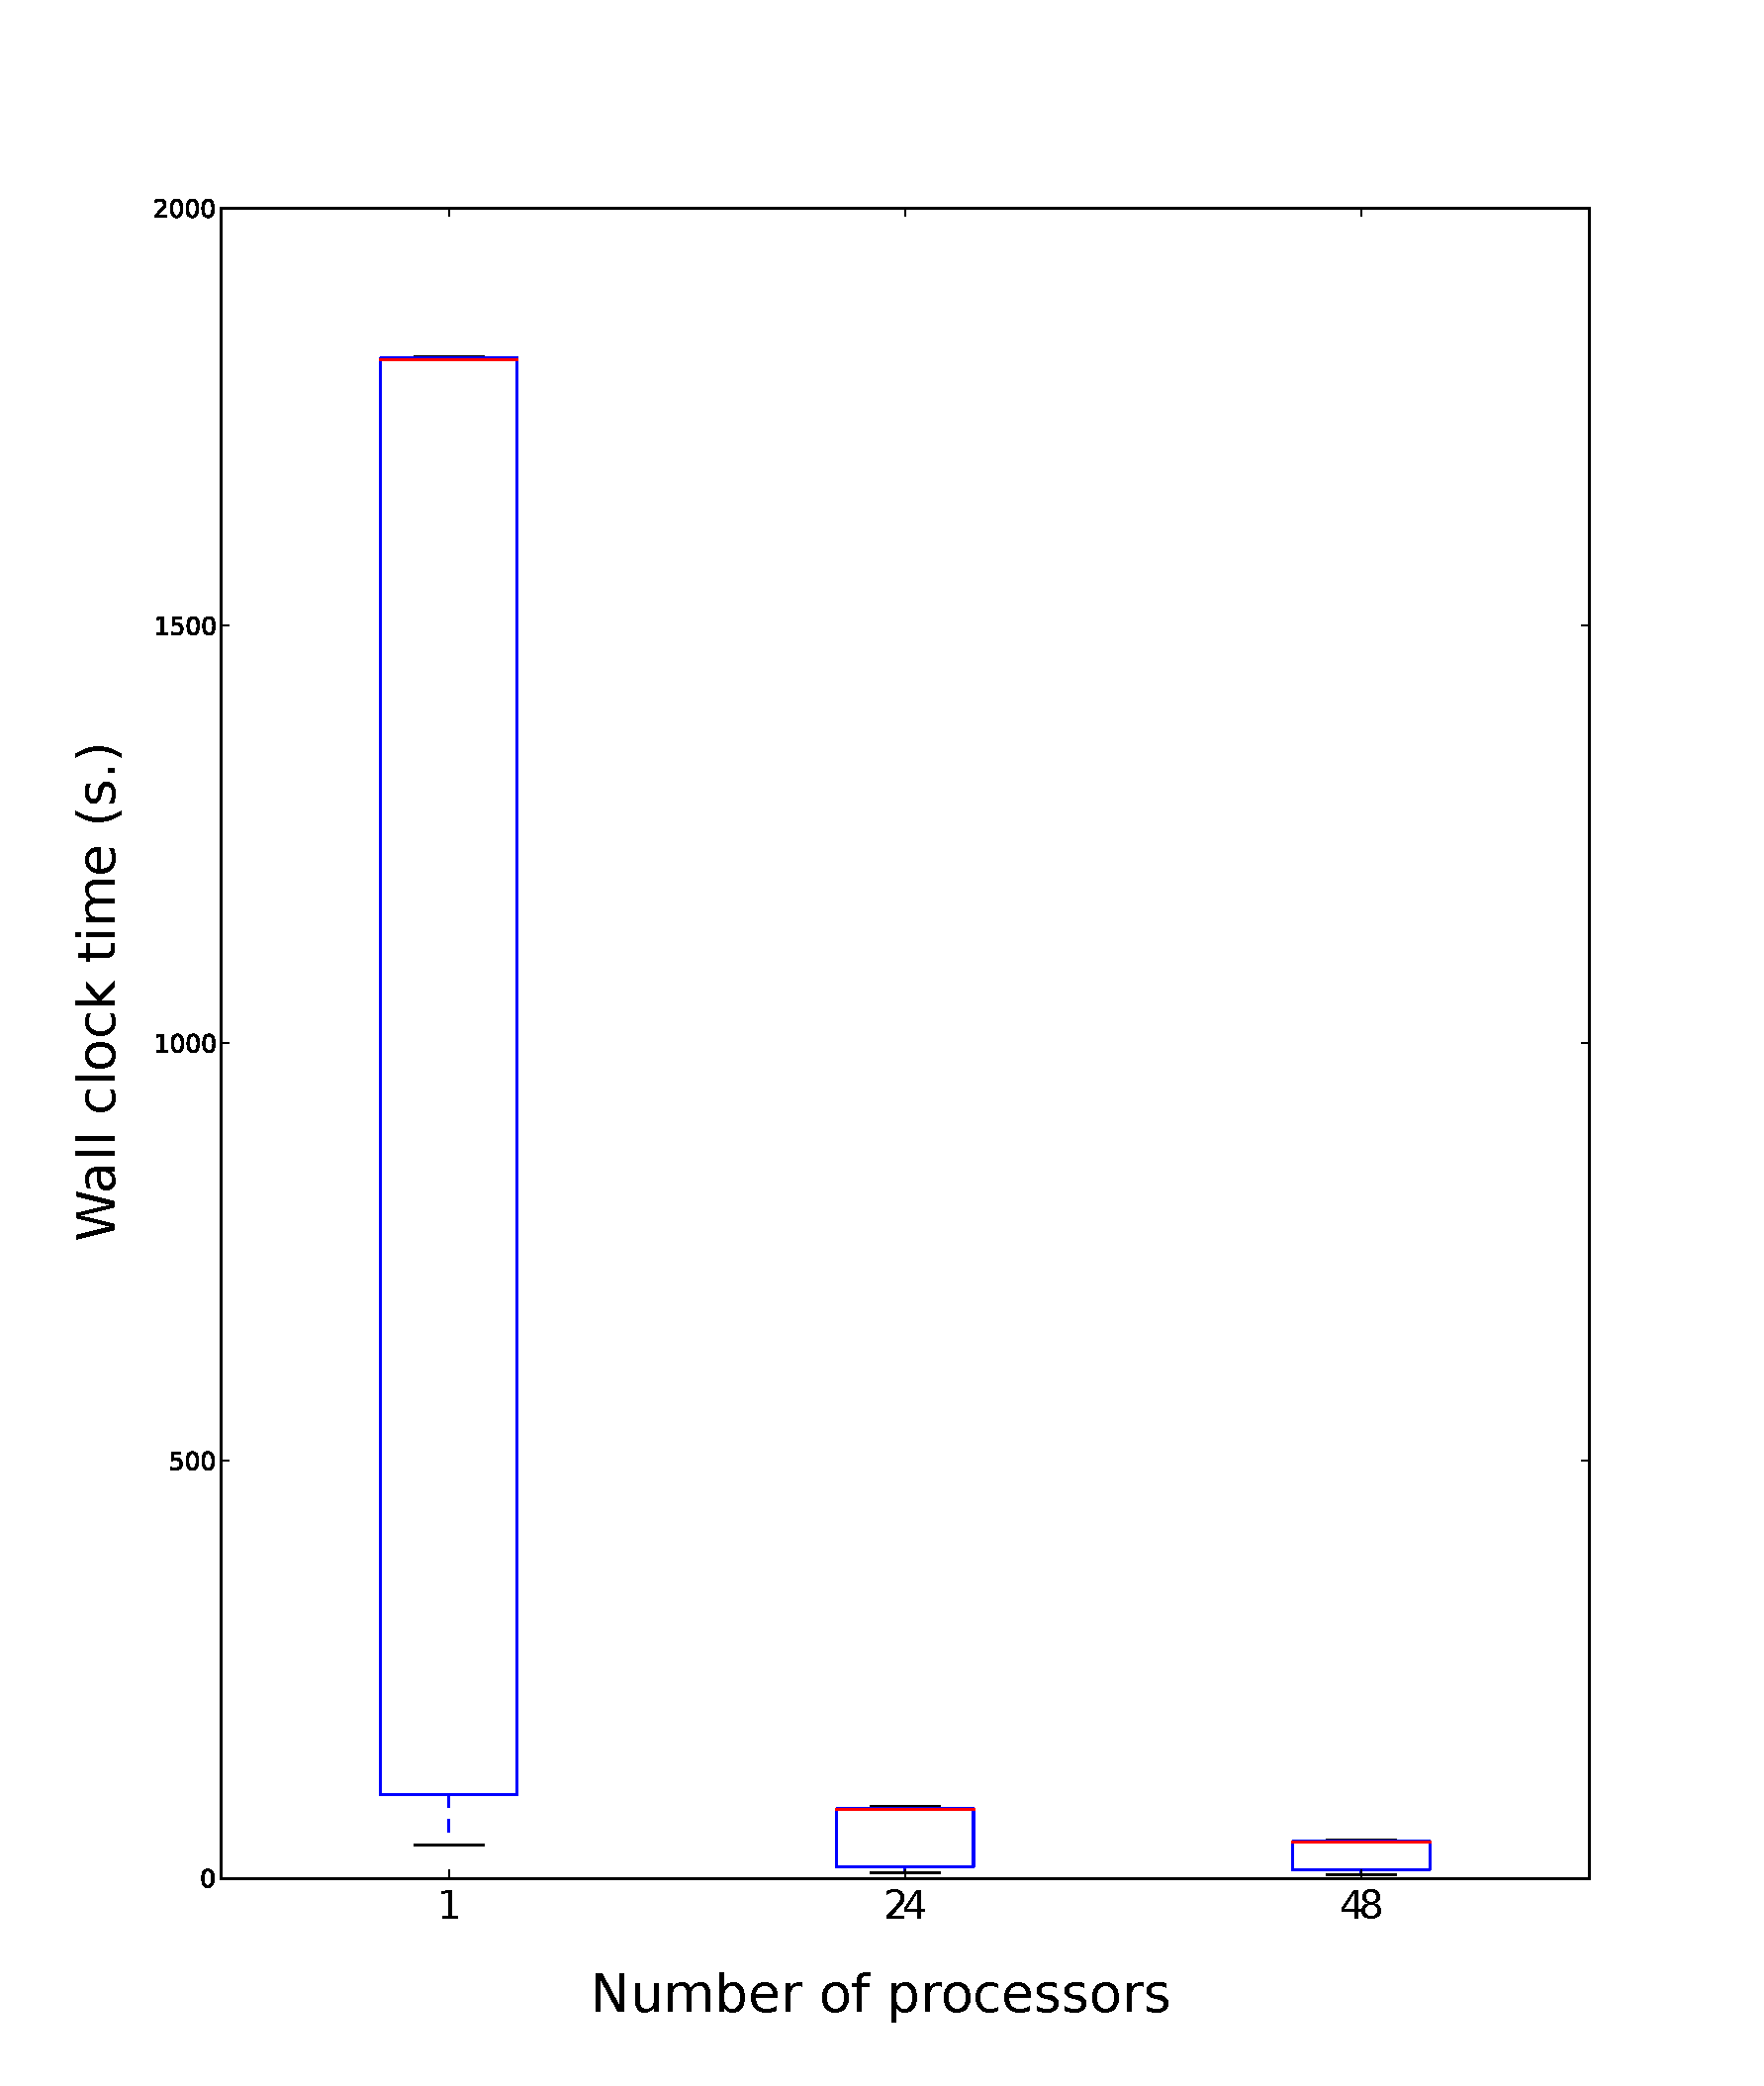
\includegraphics[width=0.2\textwidth]{images/elevators_proc_time.pdf}}
    \hfill
    \subfigure[openstacks 17]{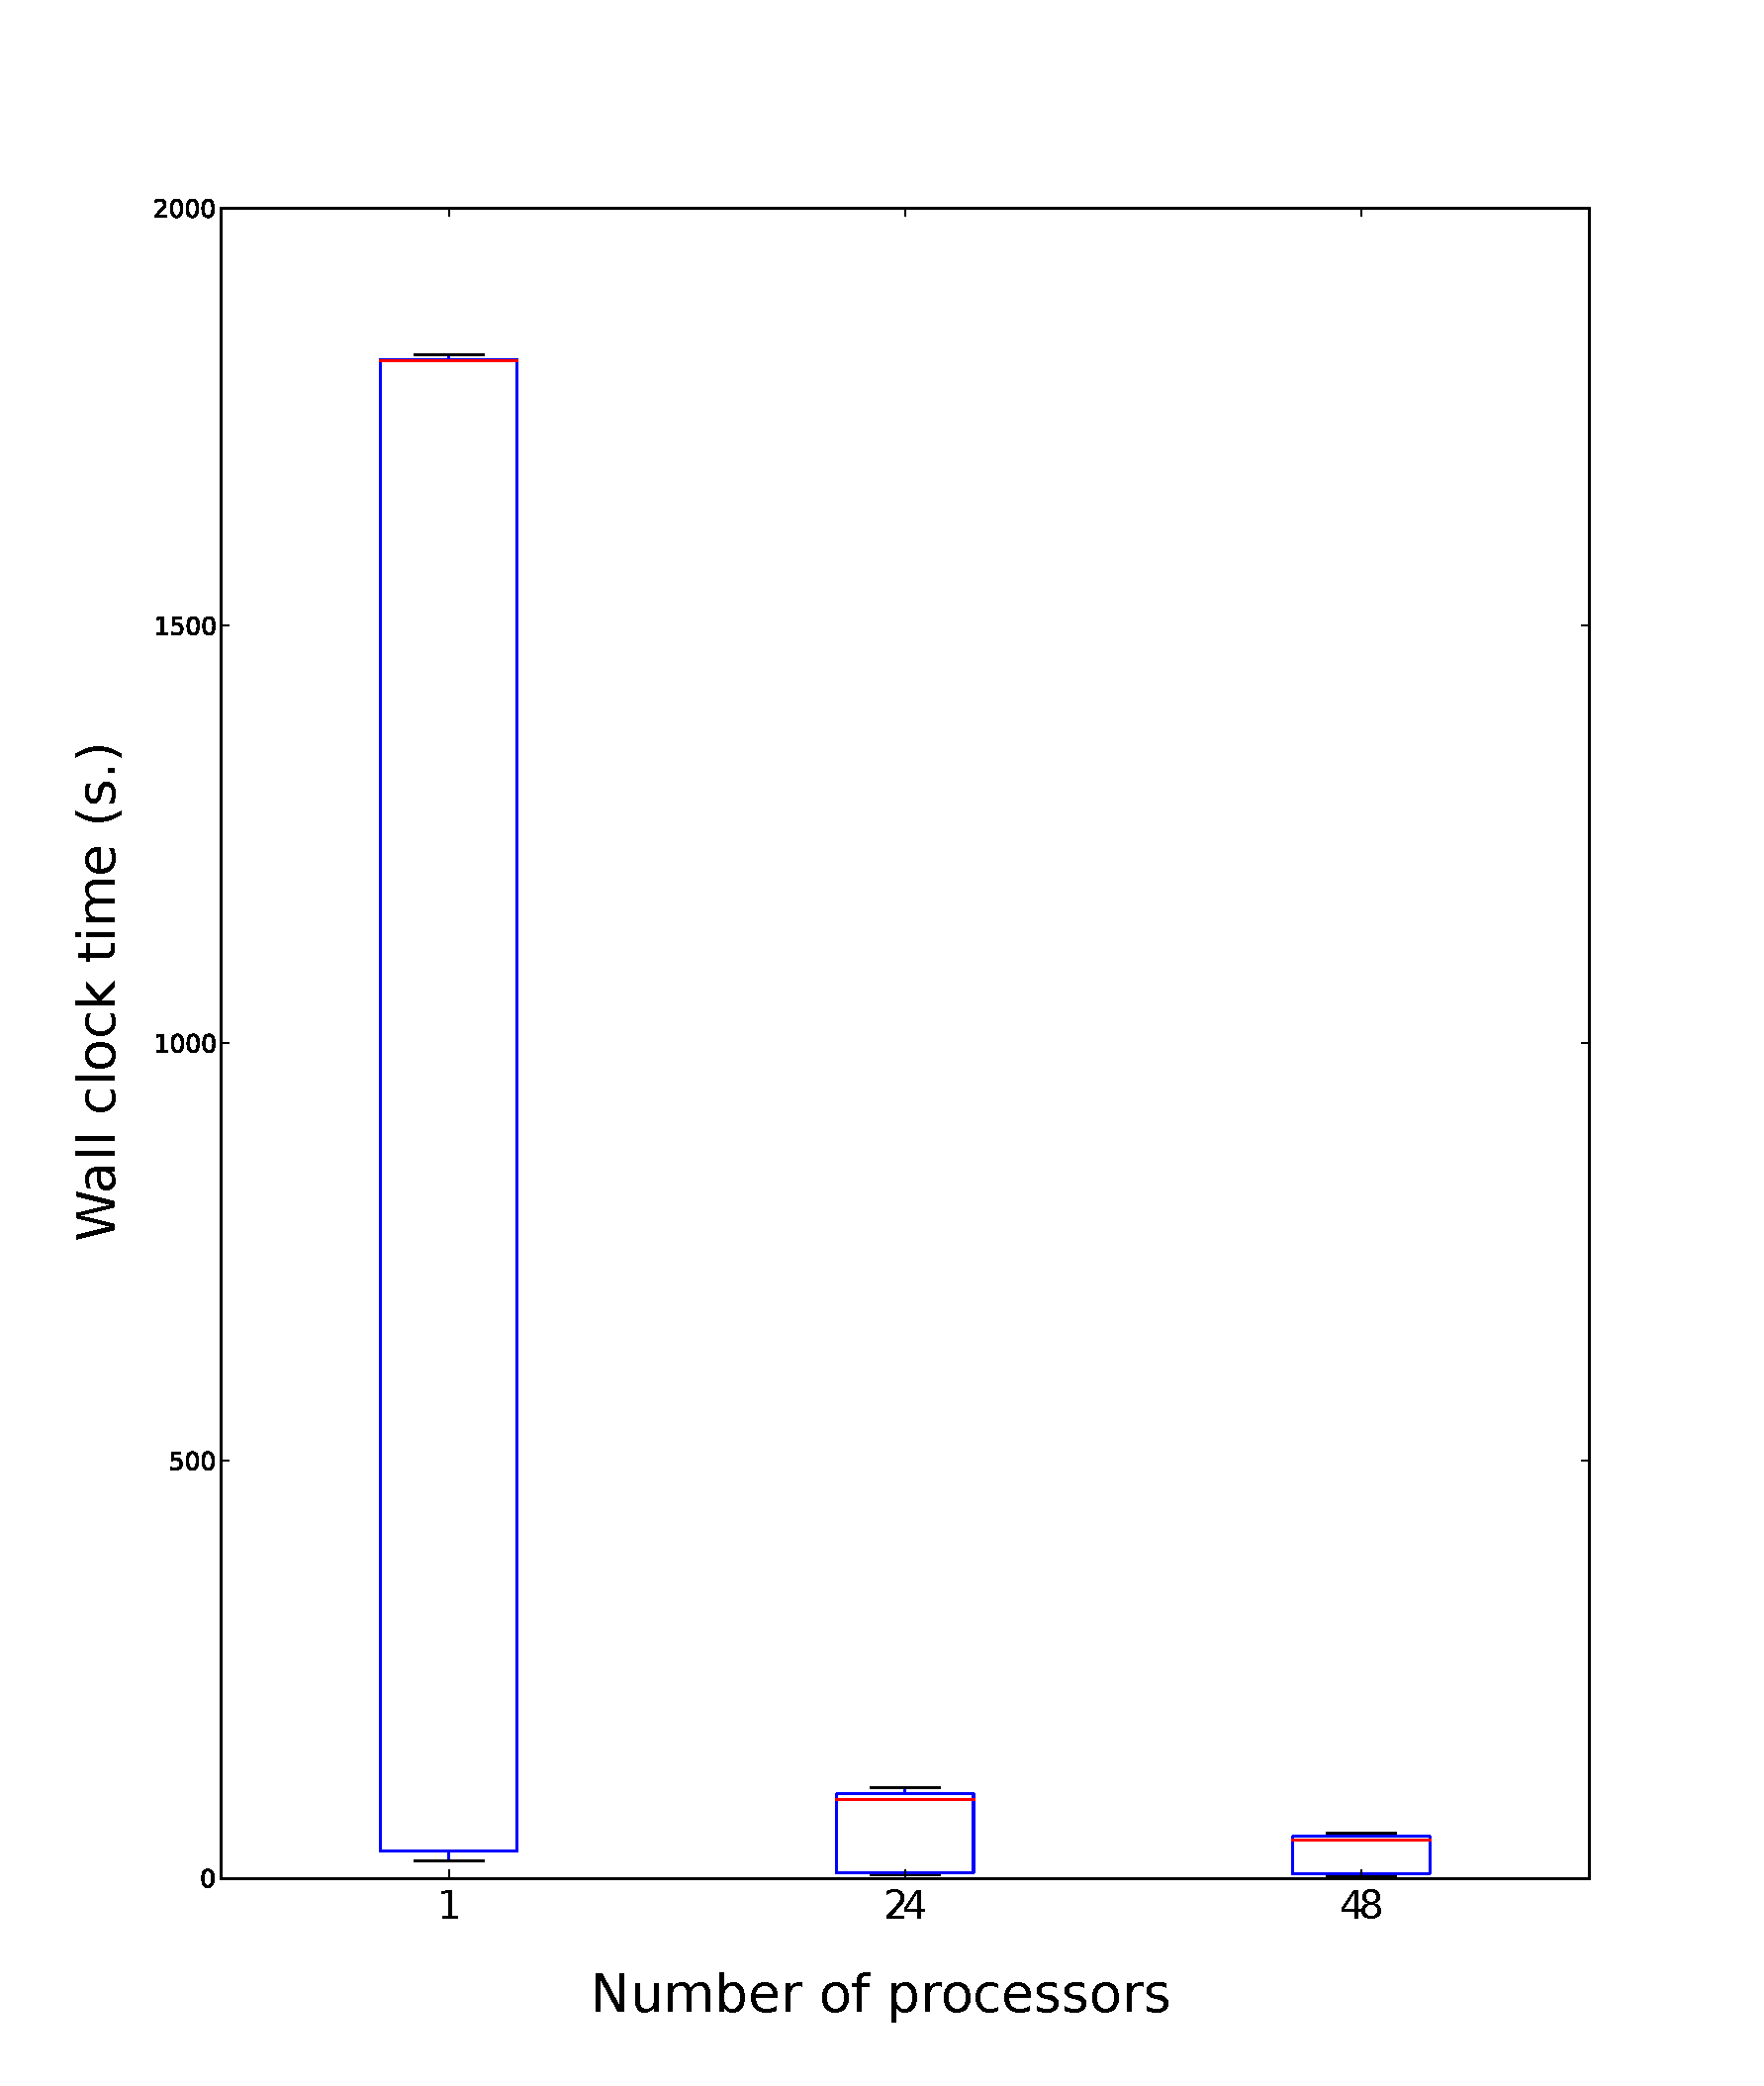
\includegraphics[width=0.2\textwidth]{images/openstacks_proc_time_dynamic.pdf}}
  \end{center}
  \caption{Absolute wallclock time distributions of 11 runs of DAE according to
  the number of processors.}
  \label{fig:proc_elevators_vs_openstacks}
\end{figure}

Figure \ref{fig:proc_elevators_vs_openstacks} shows that on both problems, the
computation time decrease with the number of processors used. Comparing to the
sequential version (running on a single processor), the parallel one permit a
decrease that is similar on both problems. The dispersions of the distribution 
is due to the steady-state stopping criterion that may be reached after different
times.

\paragraph{Comparaison of static and dynamic scheduling} % (CC, JD)

OpenMP lets the choice between the both static and dynamic task scheduling. The default one is the static scheduling.

%static scheduling

To iterate through a set of tasks we divide the number of tasks by the number of processus available. This means that each processus has some defined tasks to accomplish.

%dynamic scheduling

Regarding dynamic scheduling, during the runtime if one processus has finished these tasks it is going to work on another task available. It is similar to a tasks' queue.

% As the goal is to optimize the time cost used by a problem solved in a variable time, we have to verify whether the dynamic scheduling brings a better efficiency.

% some hypotheses

Two hypotheses have driven us to test the dynamic scheduling. The first one consists to say that as long as we are using a problem solved in a variable time, the dynamic scheduling should be faster than the static scheduling does. The second one assumes that we use a population size higher than the number of cores available, the dynamic mode should bring a better efficiency.

% less time consuming

To determine the quality of the dynamicity in front of statical schedule, we are using the following formula:

$$D_p = \frac{S^s_p}{S^d_p}$$

$S^s_p$ is the speedup for the static scheduling.\\
$S^d_p$ is the speedup for the dynamic one.\\


\begin{figure}[htpb]
  \begin{center}
    \subfigure[static]{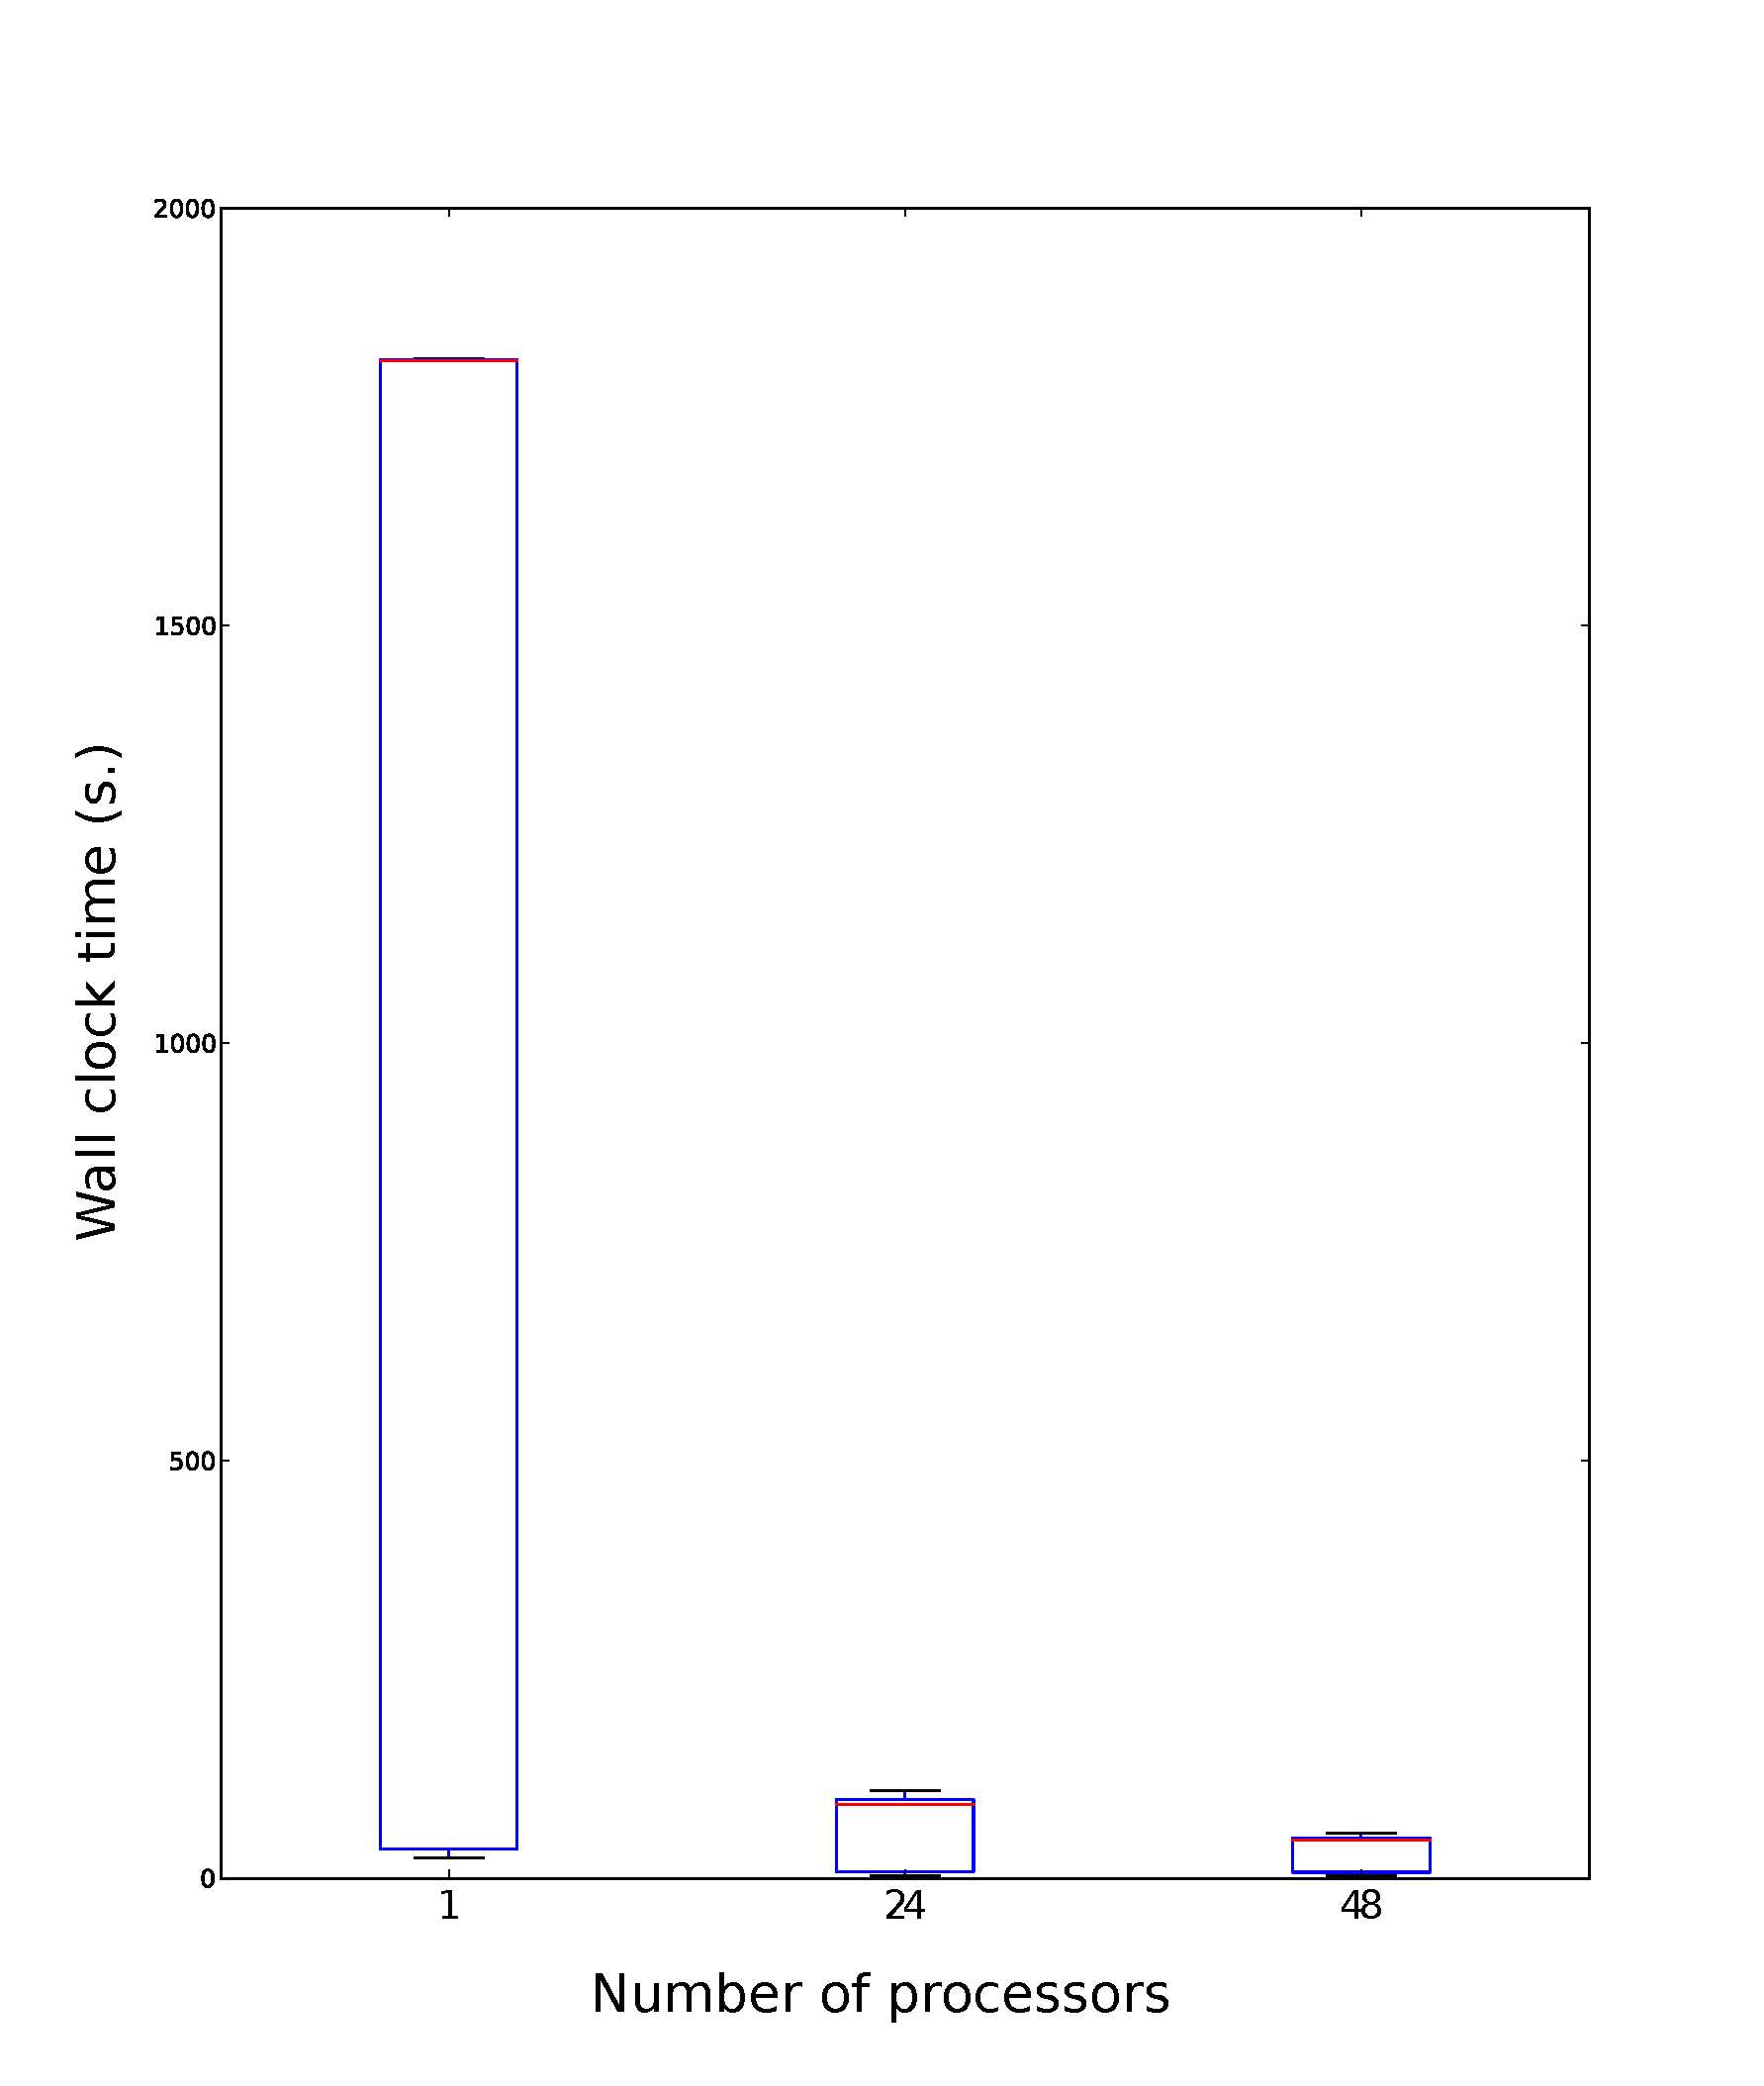
\includegraphics[width=0.2\textwidth]{images/openstacks_proc_time_static.pdf}}
    \hfill
    \subfigure[dynamic]{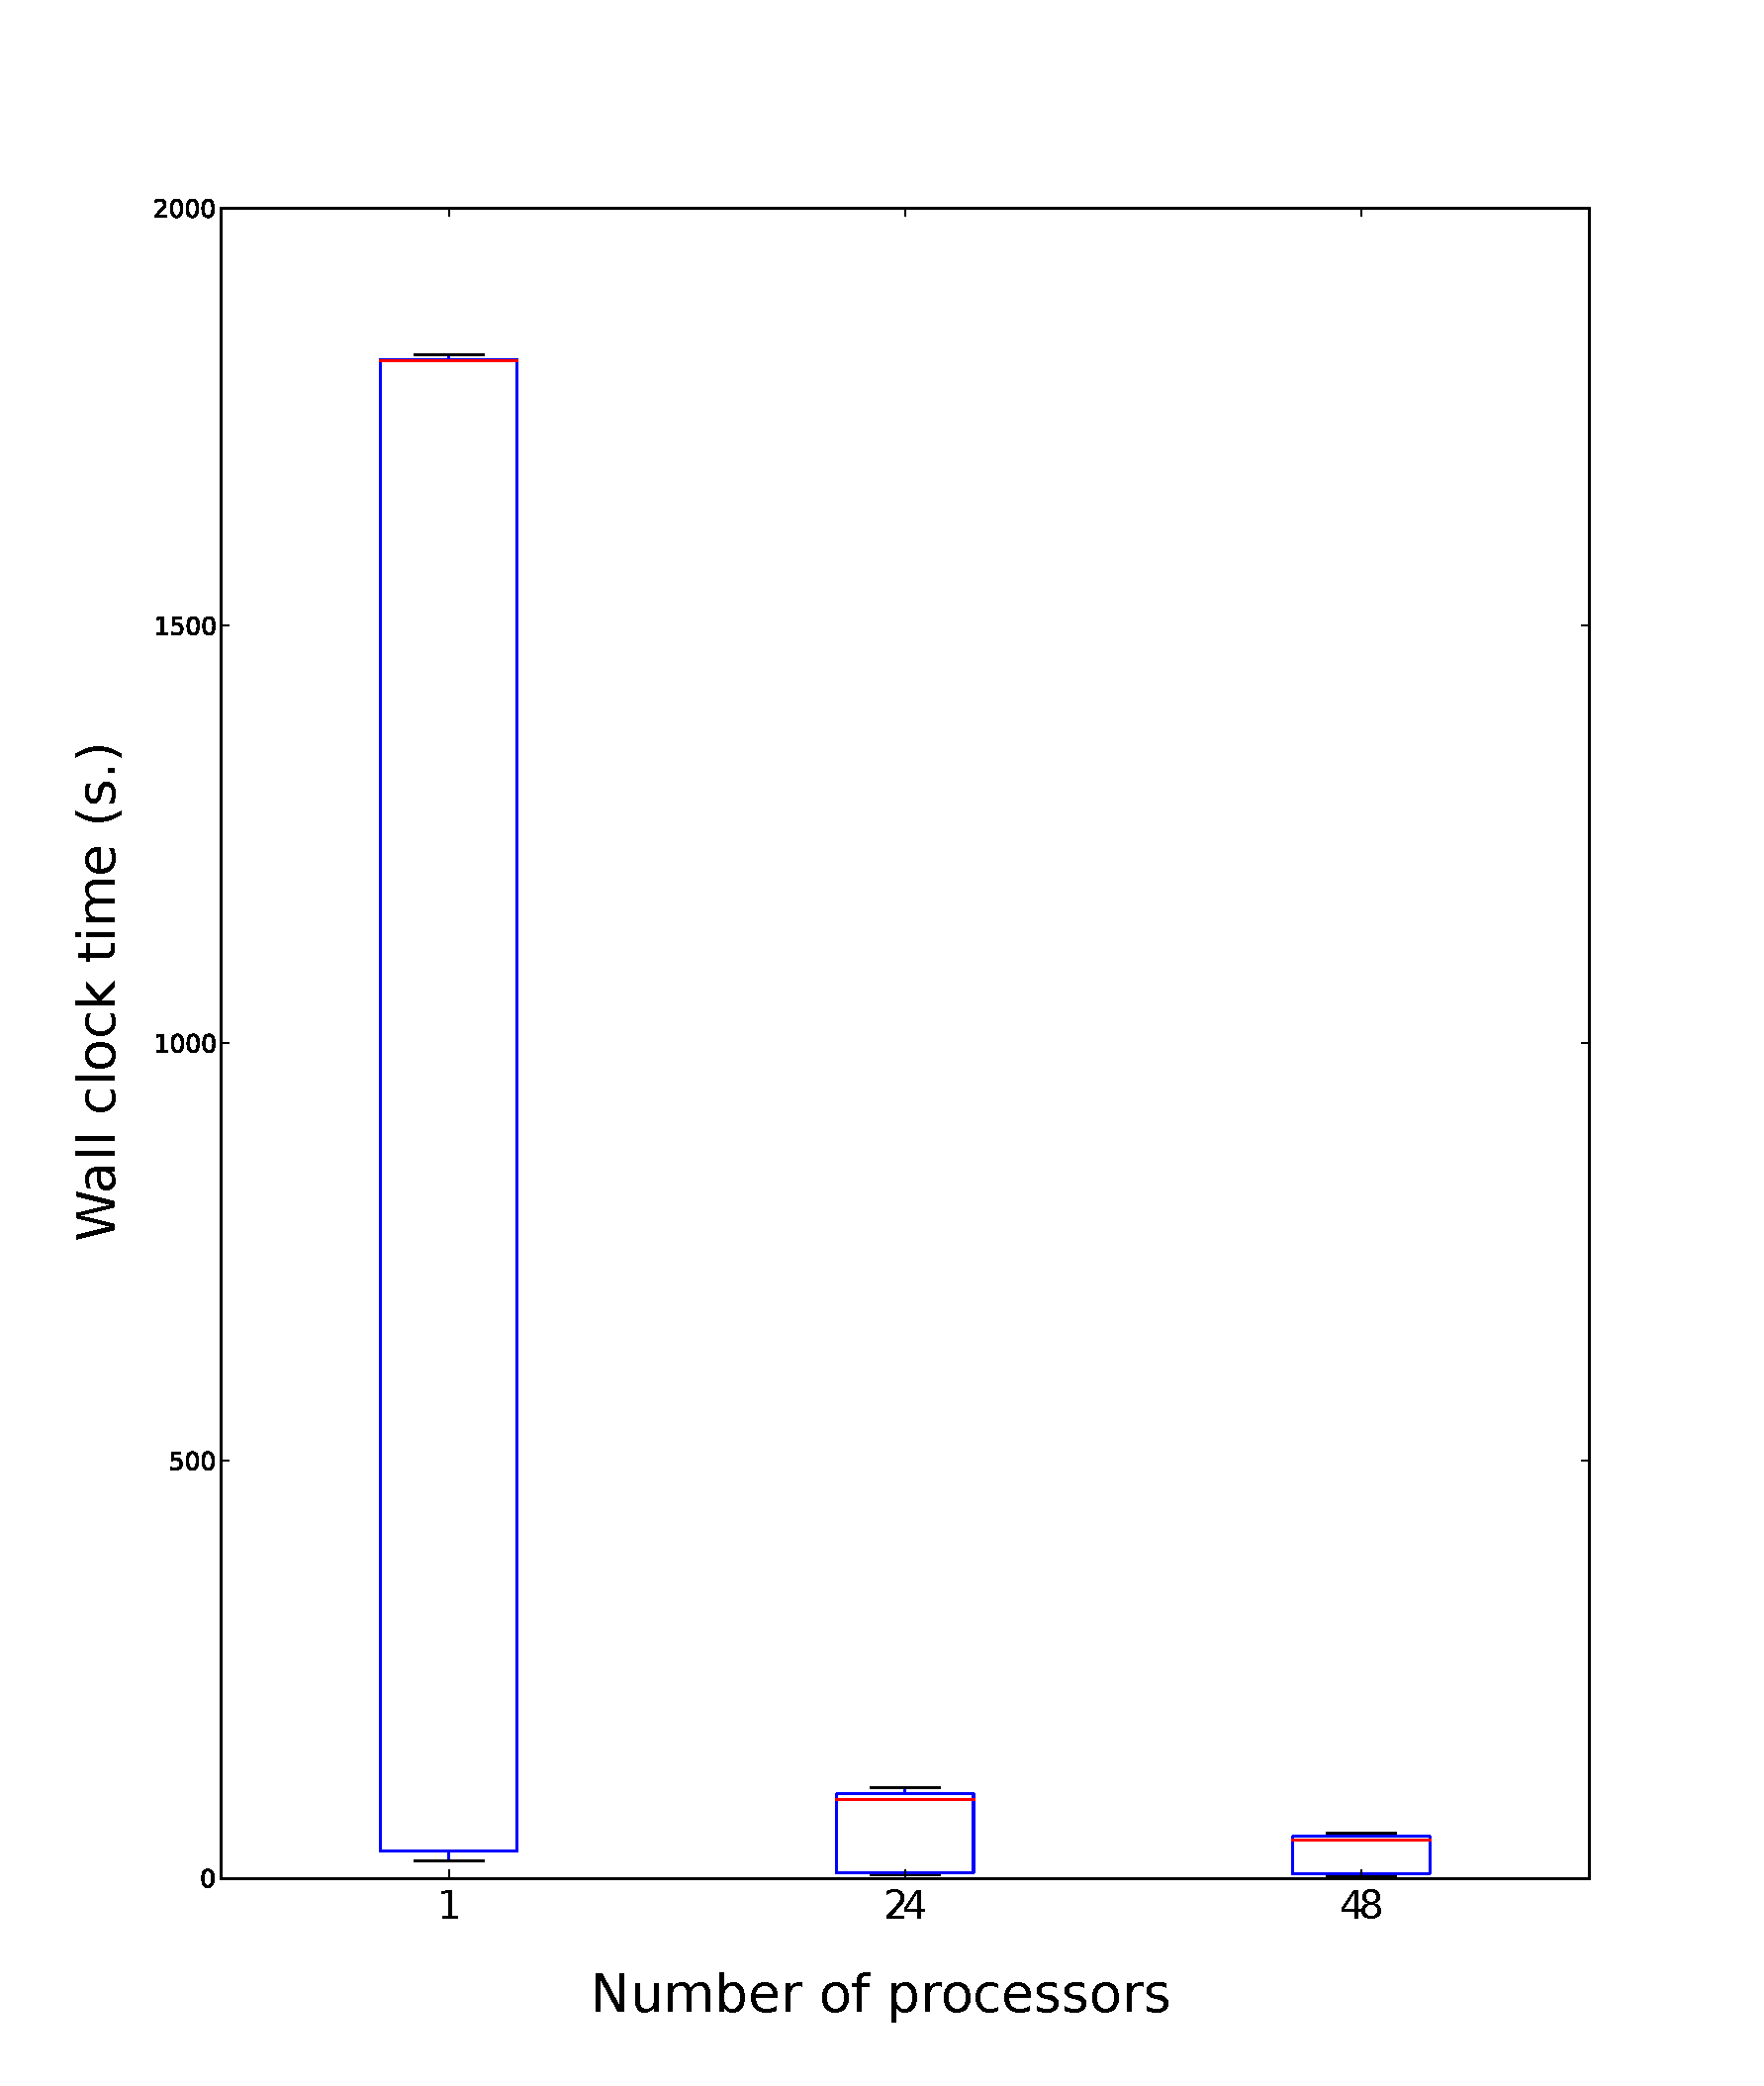
\includegraphics[width=0.2\textwidth]{images/openstacks_proc_time_dynamic.pdf}}
  \end{center}
  \caption{Absolute wallclock time distributions of 11 runs of DAE according to
  the number of processors, on the temporal openstacks-17 problem.}
  \label{fig:proc_static_vs_dynamic}
\end{figure}

Figure \ref{fig:proc_static_vs_dynamic} shows that the dynamic parallelization
scheme does not permits a significant speed-up comparing to the static one. The
Wilcoxon signed-rank test cannot reject the null hypothesis that the samples come
from the same distribution ($$p=0.03$$).

\paragraph{Speed-up against pop size} % (CC, JD)

\begin{figure}[htpb]
  \begin{center}
    \subfigure[full scale]{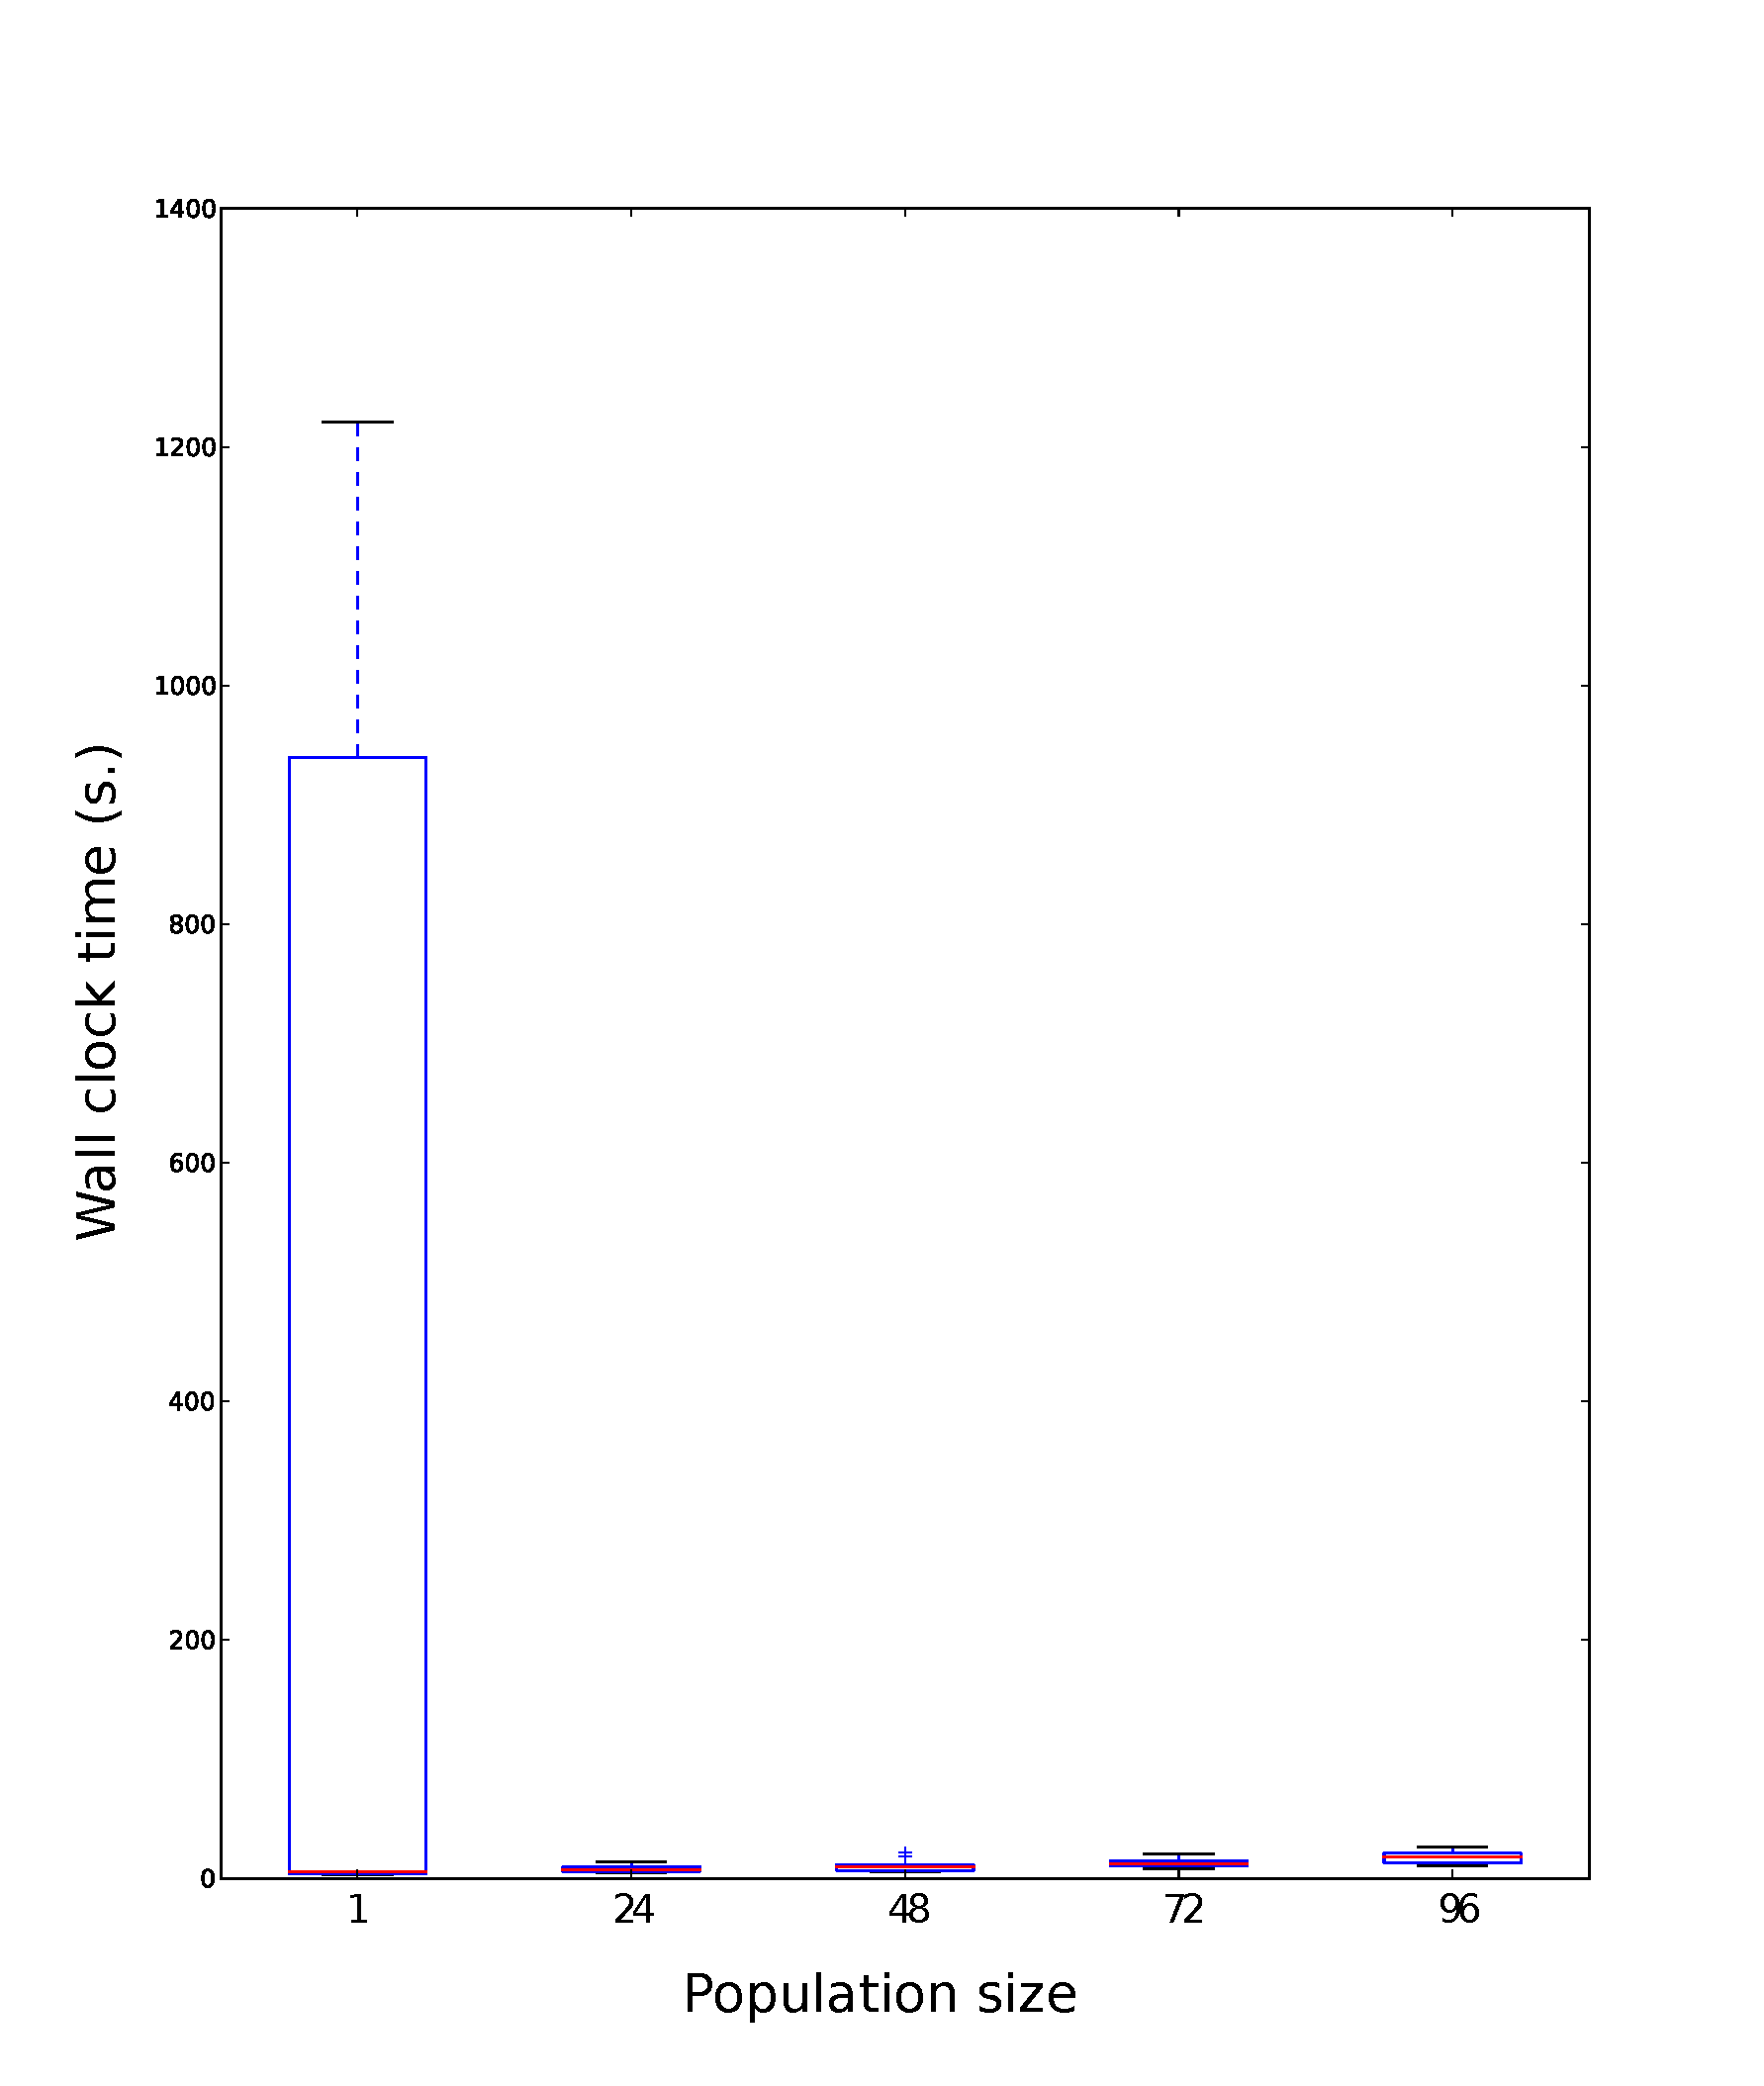
\includegraphics[width=0.2\textwidth]{images/elevators_pop_time.pdf}}
    \hfill
    \subfigure[rescaled]{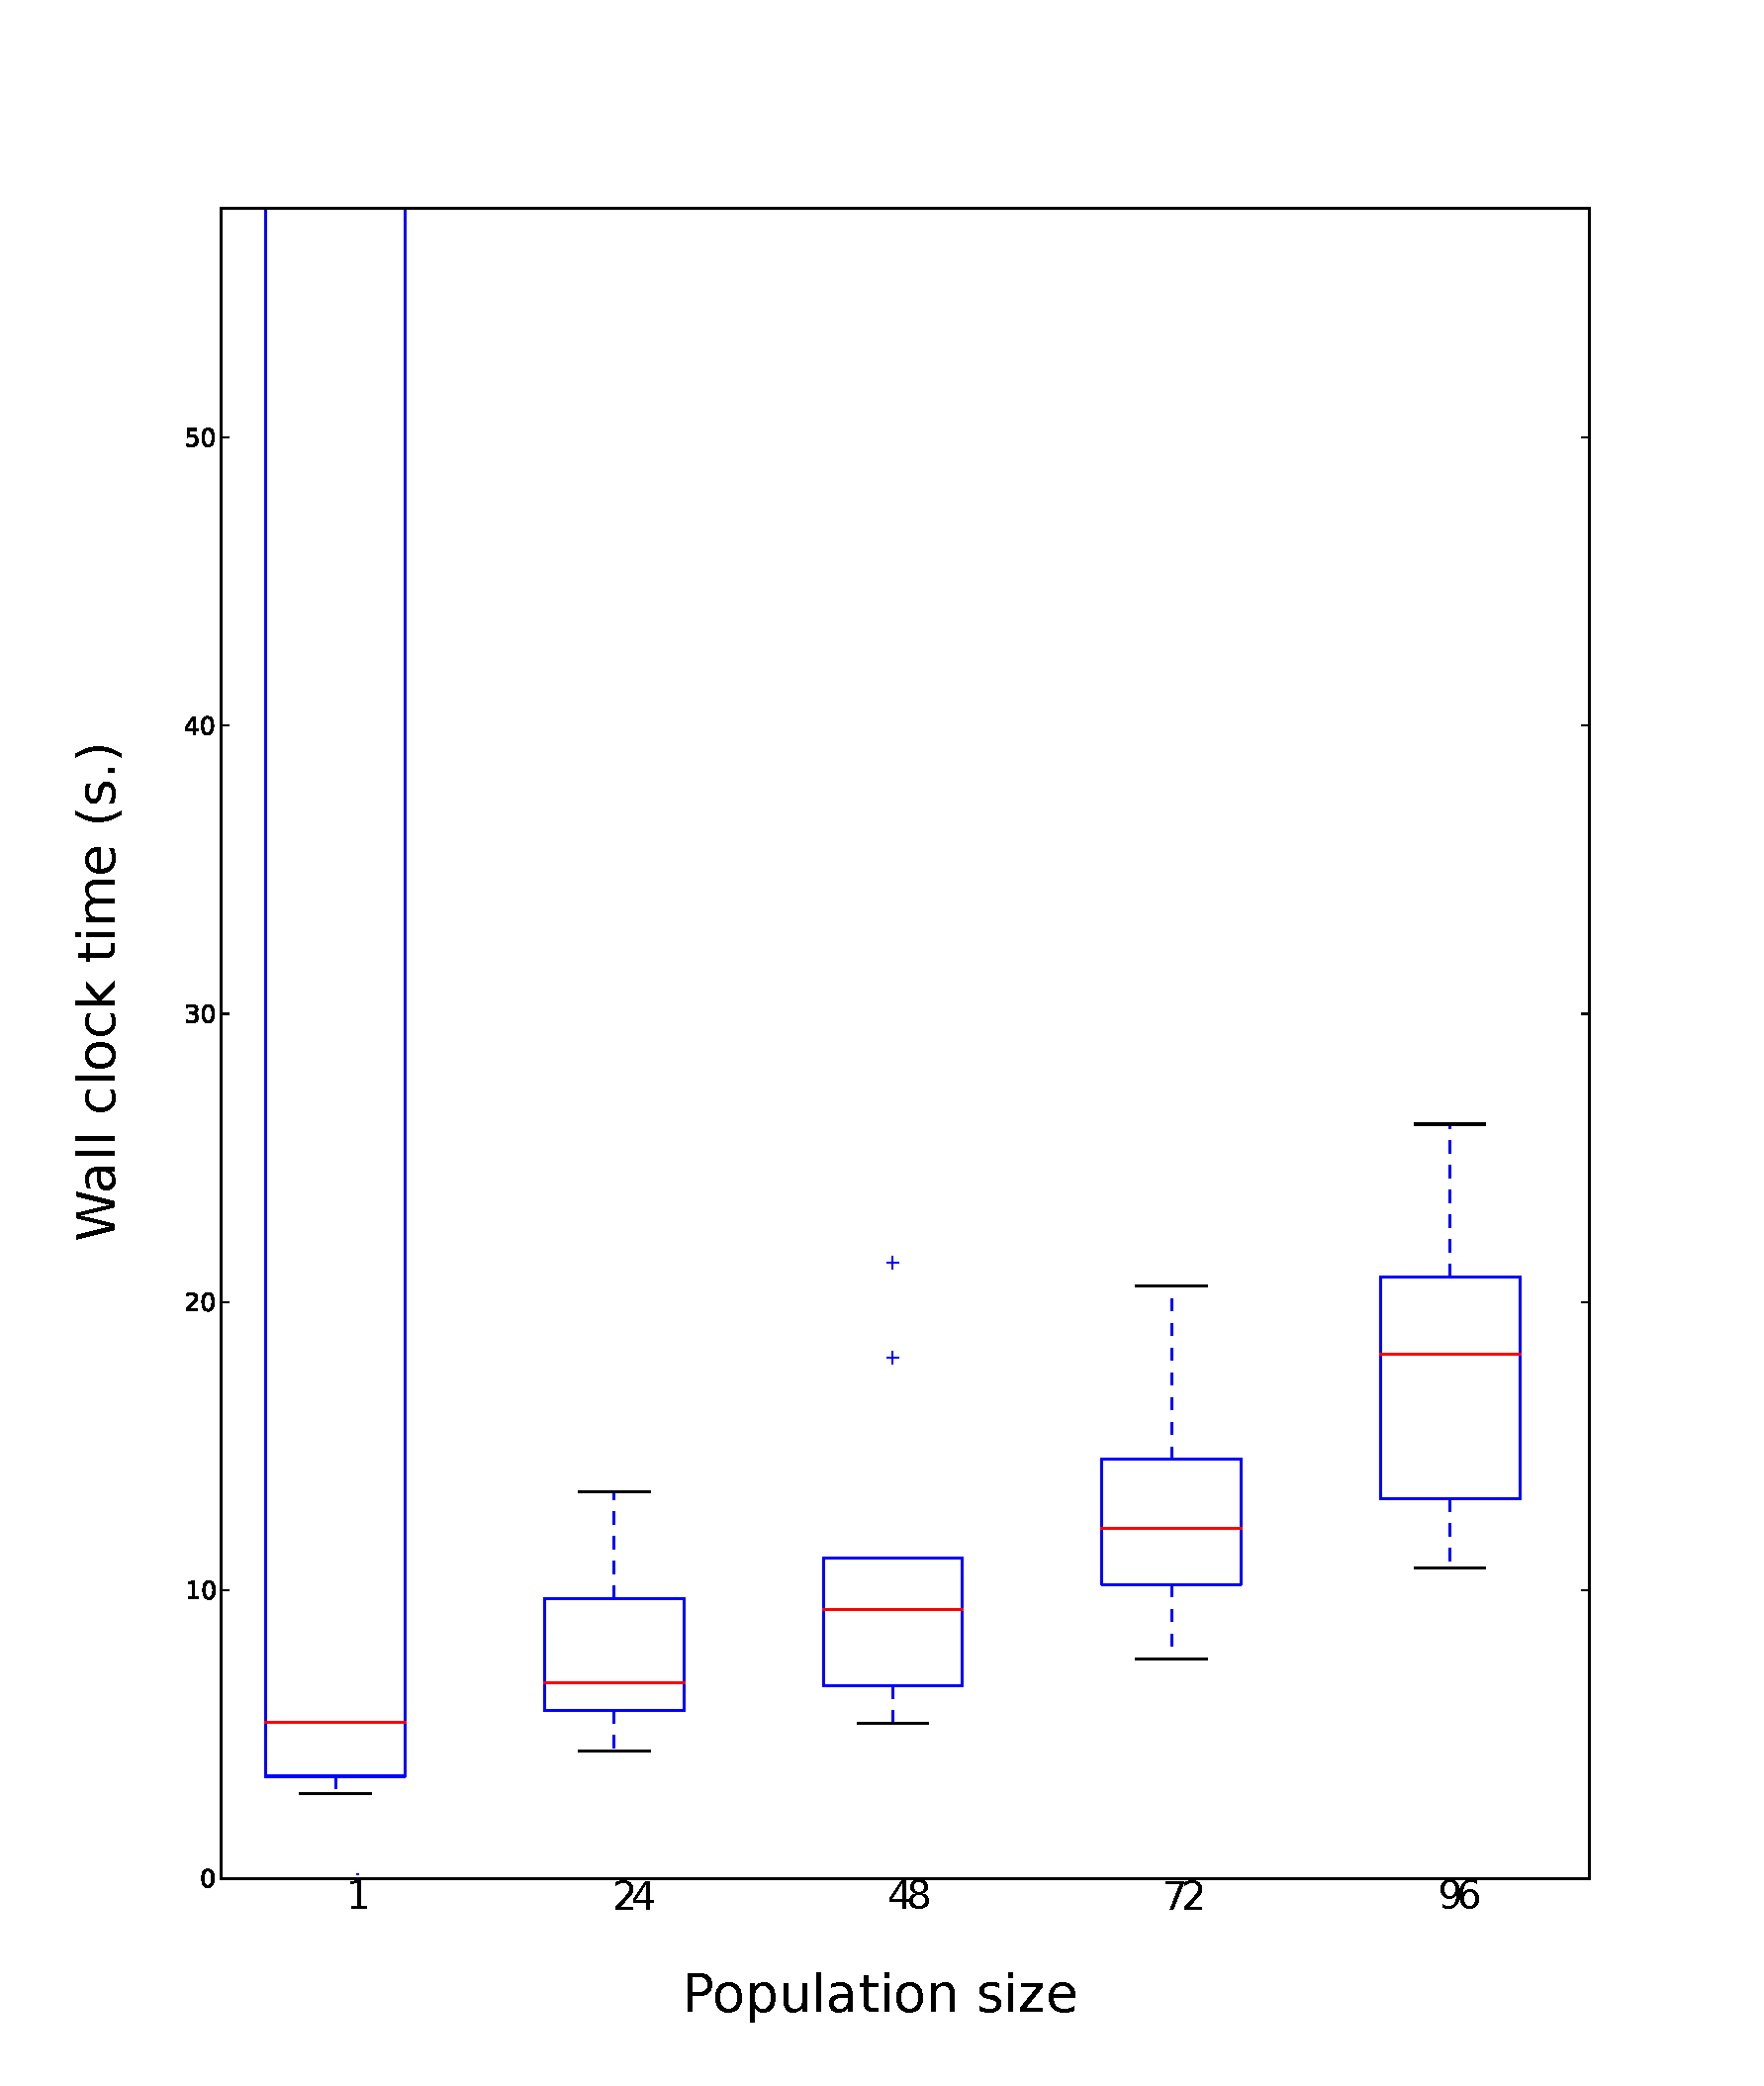
\includegraphics[width=0.2\textwidth]{images/elevators_pop_time_zoom.pdf}}
  \end{center}
  \caption{Absolute wallclock time distributions of 11 runs of DAE according to
  the population size, on the sequential elevators-12 problem, usong 48
  processors.}
  \label{fig:elevators_pop}
\end{figure}

Figure \ref{fig:elevators_pop} shows that the median computation time on a
multicore machine increase linearly with the size of the population. The 
dispersions of the distribution is due to the steady-state stopping criterion 
that may be reached after different times, with a higher probability when the
population size is small.

\section{Discussion and Conclusion}

%ACKNOWLEDGMENTS are optional
%\section{Acknowledgments}

%
% The following two commands are all you need in the
% initial runs of your .tex file to
% produce the bibliography for the citations in your paper.
\bibliographystyle{abbrv}
\bibliography{dae_mt}  % sigproc.bib is the name of the Bibliography in this case
% You must have a proper ".bib" file
%  and remember to run:
% latex bibtex latex latex
% to resolve all references
%
% ACM needs 'a single self-contained file'!
%
%Generated by bibtex from your ~.bib file.  Run latex,
%then bibtex, then latex twice (to resolve references)
%to create the ~.bbl file.  Insert that ~.bbl file into
%the .tex source file and comment out
%the command \texttt{{\char'134}thebibliography}.
\end{document}


IPC-6 ELEVATORS DOMAIN

The idea for this domain came up from the Miconic domain of IPC2, however the domain has been designed from scratch. The scenario is the following: There is a building with N+1 floors, numbered from 0 to N. The building can be separated in blocks of size M+1, where M divides N. Adjacent blocks have a common floor. For example, suppose N=12 and M=4, then we have 13 floors in total (ranging from 0 to 12), which form 3 blocks of 5 floors each, being 0 to 4, 4 to 8 and 8 to 12.

The building has K fast (accelarating) elevators that stop only in floors that are multiple of M/2 (so M has to be an even number). Each fast elevator has a capacity of X persons. Furthermore, within each block, there are L slow elevators, that stop at every floor of the block. Each slow elevator has a capacity of Y persons (usually Y<X).

There are costs associated with each elavator starting/stoping and moving. In particular, fast (accelarating) elevators have negligible cost of starting/stoping but have significant cost while moving. On the other hand, slow (constant speed) elevators have significant cost when starting/stoping and negligible cost while moving. Travelling times between floors are given for any type of elevator, taking into account the constant speed of the slow elevators and the constant acceleration of the fast elevators.

There are several passengers, for which their current location (i.e. the floor they are) and their destination are given. The planning problem is to find a plan that moves the passengers to their destinations while it maximizes some criterion.

The versions of this domain are the following:

    * Sequential: The objective function is to minimize the total cost of moving the passengers to their destinations . The total cost is increased each time an elevator starts/stops or moves.
    * Time: Each action has a duration. The goal is to minimize the makespan of the plan.
          o Time-numeric: Similar to the 'time' version; numeric fluents have been used to represent floors and capacities. 
    * Net-benefit: Having the passengers to their destinations is a soft-goal. There is a penalty associated with any passenger not being in their destination floor. The penalty is a function of the difference between the origin and the destination floor (it is supposed that the passenger with use the stairs). The objective function is to minimize the total cost expressed as a function of the cost of moving the elevators and the cost of not serving the passengers.
          o Net-benefit - numeric: Similar to net-benefit; numeric fluents have been used to represent floors and capacity constraints. 


IPC-6 OPENSTACKS DOMAIN

This domain has been used first at IPC-2006. At IPC-2008 we kept the same scenario, however we produced entirely new problem sets. So, the scenario is the following (adapted from the IPC-2006 description):

The openstacks domain is based on the "minimum maximum simultaneous open stacks" combinatorial optimization problem, which can be stated as follows: A manufacturer has a number of orders, each for a combination of different products, and can only make one product at a time.

The total required quantity of each product is made at the same time (because changing from making one product to making another requires a production stop). From the time that the first product included in an order is made to the time that all products included in the order have been made, the order is said to be "open" and during this time it requires a "stack" (a temporary storage space). The problem is to order the making of the different products so that the maximum number of stacks that are in use simultaneously, or equivalently the number of orders that are in simultaneous production, is minimized (because each stack takes up space in the production area).

The problem is NP-hard and known to be equivalent to several other problems. It was recently posed as a challenge problem for the constraint programming community (see http://www.dcs.st-and.ac.uk/~ipg/challenge/).

Note that this is an optimization problem: for any instance of the problem every ordering of the making of products is a solution, which at worst uses as many simultaneously open stacks as there are orders. Thus, finding a plan is quite trivial (in the sense that there exists a domain-specific linear-time algorithm that solves the problem), but finding a plan of high quality is hard (even for a domain-specific algorithm).

The following versions of the Openstacks domain have been used at IPC-2008:

    * Sequential: The goal is to minimize the total number of stacks. The number of stacks is represented using symbols. There are two versions of the domain in this track:
          o ADL: Universally quantified preconditions are used in order to ensure that all related orders have been started before making a product, or that all related products have been produced before shipping an order.
          o Semiground: Universally quantified preconditions have been replaced by multiple semiground actions. 
    * Time: In this case a maximum number of stacks is given and the goal is to find the plan with the least makespan, wothout violating the maximum number of stacks constraint. There are four versions of the domain in this track:
          o ADL: Similar to ADL of sequential track.
          o Semiground: Similar to semiground of sequential track.
          o ADL-numeric: Similar to ADL, but numeric fluents are used to represent the number of stacks.
          o Semiground-numeric: Similar to semiground, but numeric fluents are used to represent the number of stacks. 
    * Net-benefit: There is a cost associated with each additional stack used to make the products. Howeverm we can ship an order without all of its products beeing delivered with it. A product is considered "delivered" wrt a specific order, if the order includes the product, the product has been made and at the time the product has been made the order was open. A penalty is associated for each non-delivered product of order. There are two versions of the openstacks domain for this track:
          o ADL: Similar to ADL of the time track.
          o ADL-numeric: Similar to the ADL-numeric of the time track. 

\DAE\ has been implemented within the Evolving Objects framework (\url{http://eodev.sourceforge.net/}), an Open Source, STL-based, C++ Evolutionary Computation library. 
The fixed {\em evolution engine} is a (100+700)-ES: 100 individuals generate 700 offsprings without selection. The survival selection is performed among those 800 individuals using a {\em deterministic tournament} of size 5. For all runs, the {\bf stopping criterion} is the following: After at least 10 generations, evolution is stopped if no improvement of the best fitness in the population is made during 50 generations, with a maximum of 1000 generations. Furthermore, all runs were allowed a maximum CPU time of 30mn (running on 3.4 GHz cores).\\
